\chapter{Evaluation of OpenVINO and the Myriad X VPU with Error-Tolerant Applications when Applying Algorithmic Transformations}
\label{ch:ch1}

\section{Overview}

%This chapter explores the performance impact of how substituting a region of imperative code with a trained neural network that provides the same functionality in an approximate way. This area of approximate computing was previously explored in slightly different ways, utilizing code annotation to substitute the annotated piece of code with an inference call to a neural network. In \cite{Esmaeilzadeh2012}, an implementation is done by simulating an NPU that runs next to the CPU and at the same frequency. In \cite{Moreau2015a} and \cite{Moreau2015}, the inference is run in an FPGA which runs at one-fourth of the frequency of the CPU. In both cases the NPU is tightly coupled with the CPU.

The main objective of the work presented in this chapter is to explore the performance when doing approximate computing with neural networks utilizing OpenVINO, a free toolkit, as well as testing the capabilities of the Intel Neural Compute Stick 2 and the Movidius Myriad X VPU. This is a loosely coupled solution, it sacrifices latency and throughput for the flexibility of a plug-and-play device. The idea is to try to replicate what was done at an academic level and reproduce it in an environment with off-the-self components.

This chapter will focus on five applications from the AxBench suite of error-tolerant applications: blacksholes, inversek2j, jmeint, kmeans and sobel. The Black-Scholes model is a mathematical model for the dynamics of a financial market. Inversek2j is used in robotic and animation, it computes the angles of 2-joint robotic arms. Jmeint is a 3D gaming workload it determines if a pair of triangle coordinates intersect. Kmeans partitions a set of input points into a number of clusters. Sobel takes a color image and produces a gray-scale image highlighting the edges \cite{Yazdanbakhsh2016}.

\section {Tested Platforms Details}

Three different platforms were tested to obtain results on the selected applications: a desktop PC with an Intel CPU, a Raspberry Pi 3 Model B and a Raspberry Pi 4 Model B. Table \ref{tab:hw_sw_details} shows the details of each platform and Figure \ref{fig:phys_setup} shows pictures of the three platforms. For the neural network processing, the Intel Neural Compute Stick 2 was utilized.

These platforms were selected to have a range of different computing power. The low power Myriad X VPU will be compared against a powerful desktop CPU but also against much energy efficient systems like the ARM CPUs that the Raspberry Pi models include. For these experiments other compute devices could have been chosen, such as GPUs or FPGAs. The focus of this thesis is to evaluate a readily available low power off-the-shelf device like the NCS2 than can be paired with similar low power devices such as the Raspberry Pi, which are relevant nowadays with the growing importance of edge computing and Internet of Things (IoT).

\begin{table}[thbp]
\centering
\caption{Platform details.}
\label{tab:hw_sw_details}
\resizebox{\textwidth}{!}{%
\begin{tabular}{|l|l|l|l|l|l|l|}
\hline
\multicolumn{1}{|c|}{\textbf{Platform}}                          & \multicolumn{1}{c|}{\textbf{CPU}}                                                      & \multicolumn{1}{c|}{\textbf{GPU}}                                         & \multicolumn{1}{c|}{\textbf{RAM}}                             & \multicolumn{1}{c|}{\textbf{USB Ports}}               & \multicolumn{1}{c|}{\textbf{OS}}                                                              & \multicolumn{1}{c|}{\textbf{OpenVINO}} \\ \hline
Desktop PC                                                       & \begin{tabular}[c]{@{}l@{}}Intel Core i7-5930K\\ 6 C / 12 T\\ 3.5-3.7 GHz\end{tabular} & \begin{tabular}[c]{@{}l@{}}Nvidia\\ GTX 980\end{tabular}                  & \begin{tabular}[c]{@{}l@{}}16 GB DDR4\\ 2133 MHz\end{tabular} & \begin{tabular}[c]{@{}l@{}}USB 3\\ USB 2\end{tabular} & \begin{tabular}[c]{@{}l@{}}Ubuntu 20.04\\ \\ Kernel 5.4\end{tabular}                          & 2020.1                                 \\ \hline
\begin{tabular}[c]{@{}l@{}}Raspberry Pi 3\\ Model B\end{tabular} & \begin{tabular}[c]{@{}l@{}}Cortex-A53\\ 4 Cores\\ 1.2 GHz\end{tabular}                 & \begin{tabular}[c]{@{}l@{}}Broadcom\\ VideoCore IV\\ 250 MHz\end{tabular} & 1 GB                                                          & USB 2                                                 & \begin{tabular}[c]{@{}l@{}}Raspberry Pi OS\\ version 2020-05-27\\ \\ Kernel 4.19\end{tabular} & 2020.1                                 \\ \hline
\begin{tabular}[c]{@{}l@{}}Raspberry Pi 4\\ Model B\end{tabular} & \begin{tabular}[c]{@{}l@{}}Cortex-A72\\ 4 Cores\\ 1.5 GHz\end{tabular}                 & \begin{tabular}[c]{@{}l@{}}Broadcom\\ VideoCore IV\\ 500 MHz\end{tabular} & 4 GB                                                          & \begin{tabular}[c]{@{}l@{}}USB 3\\ USB 2\end{tabular} & \begin{tabular}[c]{@{}l@{}}Raspberry Pi OS\\ version 2020-05-27\\ \\ Kernel 4.19\end{tabular} & 2020.1                                 \\ \hline
\end{tabular}%
}
\end{table}

\begin{figure}[thbp]
	\centering
	\includegraphics[scale=0.75]{phys_setup}
	\caption{Physical setup for the tested platforms: Desktop PC, Raspberry Pi 4, Raspberry Pi 3.}
	\label{fig:phys_setup}
\end{figure}

\section{Methodology, Workflow and Implementation Details}

The whole purpose of the experiments run for this chapter is to have two versions for each application: one that runs the original imperative code in the CPU and another version that substitutes part of the code with a call to a neural network and that utilizes OpenVINO to do the inference on a supported device. This was achieved using the workflow shown in Figure \ref{fig:workflow}.

\begin{figure}[thbp]
	\centering
	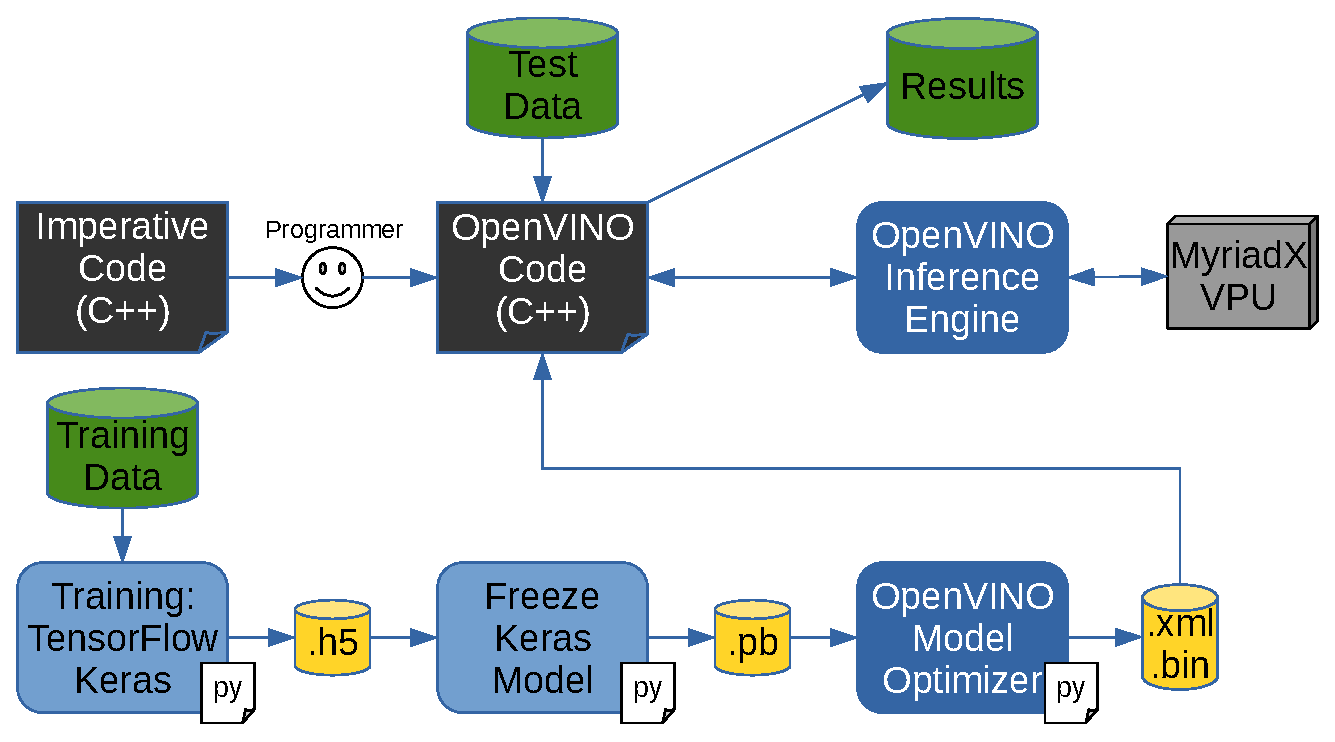
\includegraphics[scale=0.75]{workflow}
	\caption{Diagram of the workflow to apply the algorithmic transformation technique for approximate computing using the OpenVINO toolkit.}
	\label{fig:workflow}
\end{figure}

The starting point for this was the AxBench code for the applications that are going to be tested. AxBench is a general, diverse, and representative  set of benchmarks to evaluate different approximate computing techniques \cite{Yazdanbakhsh2016}. Since the benchmarks included in AxBench have been used in other relevant papers referenced by this work it was decided that it was the best set of applications to use as a baseline, that way it can be easily compared against previous works. These were selected because they represent a varied range of real-world error-tolerant applications from a wide range of domains. These applications are in line with evaluations done in previous work on approximate computing. Each application was written in procedural C++ originally. They will be re-written using an algorithmic transformation where a section of the code will be substituted to a call to run a neural network that will approximate the computations of the substituted code. For each of the applications the performance will be measured and compared against the original non-approximate application. The error for each of the applications will also be measured to see how much the results from the approximate version deviate from the non-approximate original version.

In the original AxBench applications whenever the user wants to substitute part of the code with an inference call, an annotation on the code is done and that will be substituted with a single call to the NPU. To be able to utilize OpenVINO's full potential the applications had to be modified to support batch processing. Instead of calling the inference on each iteration, the inputs to the neural network are stored in a buffer and when the buffer is filled a single call is made and all the stored inputs are all processed by a single inference call by OpenVINO. There are two main reasons to do it this way. One is that OpenVINO is a toolkit specialized for image processing and thus, optimized to handle CNNs. The same is true for the Myriad X VPU, the best performance is provided when the data is handled in batches in the form of a CNN. The second reason is that there is an overhead when sending the data to the device that is doing the inference. When utilizing the CPU for inference the overhead might not be as critical, but when utilizing a device like the NCS2, the input data needs to travel through an USB bus to the device and the output data needs to travel back to the PC and copied to the output buffer.

Creating and training the neural networks for the applications was done using Tensorflow version 1.15, the latest one compatible with OpenVINO version 2020.1. After training, the neural network is saved in a Keras \textit{.h5} format. To be able to load the network in OpenVINO this needs to be converted to OpenVINO's Intermediate Representation (IR). The \textit{.h5} format can't be converted directly, so a script is used to freeze the model and save it as a \textit{.pb} Tensorflow file, which can be used by OpenVINO's Model Optimizer to transform the model into the IR, which consists of a .bin and a .xml file, these contain the weights and biases and the topology of the network respectively. All applications were trained for a total of 1000 epochs.

As mentioned before, OpenVINO and the Myriad X VPU perform the best when processing the data in parallel in the form of a CNN. This means that for each application instead of handling one inference at a time as a fully connected network, multiple inferences are handled by emulating a multi-input fully connected networks as a CNN. For example, let us say that there is a fully connected neural network with an input of size 3, an output of size 2 and a hidden layer of size \textit{X}. This would be implemented in Tensorflow as a model with an input of three neurons, a hidden dense layer of \textit{X} number of neurons and an output dense layer with two neurons. To implement the same topology but in a CNN way where the network could process many inputs at a time, the first layer would be a 2D-convolutional layer with kernel of size (height=1, width=3), a stride of size (vertical=1, horizontal=3) and an output of \textit{X} channels, that connects to another 2D-convolutional layer now with kernel and stride both of size (1, 1) and an output size of 2 channels.

The code in Listing \ref{lst:code_dense} defines a fully-connected neural network with topology 3-X-2. All layers are using the Relu activation function.

\begin{minipage}{\linewidth}
\begin{lstlisting}[frame=single, tabsize=4, caption={Tensorflow example model using dense layers.},label={lst:code_dense},language=Python,captionpos=b]
	model = Sequential()
	model.add(Dense(X, activation='relu',
	                   input_shape=(3,)))
	model.add(Dense(2, activation='relu'))
\end{lstlisting}
\end{minipage}

The same topology can be created as a CNN, this time several neural networks are created, which allows for parallel inference. In the Listing \ref{lst:code_dense} example the input shape was a trivial one-element tuple with the number of inputs (3). In the CNN case, shown in Listing \ref{lst:code_cnn}, the matrix has a BxB size, so the input shape has height=B, width=Bx3 (the number of inputs for a single sample is 3) and channels=1. The hidden layer is a CNN layer with \textit{X} number of channels and has a simple (1,1) kernel and stride. The output is a 2-channel layer. The padding value `valid' means that no padding is added to the layer.

\begin{minipage}{\linewidth}
\begin{lstlisting}[frame=single, tabsize=4, caption={Tensorflow example model using convolutional layers.},label={lst:code_cnn},language=Python,captionpos=b]
	model = Sequential()
	model.add(Conv2D(X, (1,3), strides=(1,3),
	                           padding='valid',
	                           activation='relu',
	                           input_shape=(B,B*3,1)))
	model.add(Conv2D(2, (1,1), strides=(1,1),
	                           padding='valid',
	                           activation='relu'))
\end{lstlisting}
\end{minipage}

It is important to note that for this exploration each application was modified manually to be able to run with OpenVINO, this is because each one was implemented differently and it is not the objective of this exploration to automate the process of identifying the piece of code and creating the OpenVINO compatible inference calls nor training the neural networks automatically. Nonetheless, the following simplified code snippets show the basic ideas of how to implement the inference solution using the OpenVINO toolkit.

The code snippet in Listing \ref{lst:orig_code} shows the original procedural code. A simple loop iterates over all the inputs and for each one of them a error-tolerant function is called. The result is saved in an outputs array.

\begin{minipage}{\linewidth}
\begin{lstlisting}[frame=single, tabsize=4, caption={Procedural code of an error-tolerant function.},label={lst:orig_code},language=Python,captionpos=b]
	for (int i = 0; i < inputs.size(); i++) {
		outputs[i] = ErrorTolerantFunction(inputs[i]);
	}
\end{lstlisting}
\end{minipage}

The next code snippet shown in Listing \ref{lst:naive_code} uses a naive implementation of the code where a simple fully-connected neural network is used. The code execution is extremely slow when using OpenVINO and the NCS2 because for each input the data needs to travel through the USB3 bus, then the Myriad X does the inference and finally the data needs to travel back, which introduces latency on each call. For these simplified examples the assumption is that the neural network has one input and one output, hence the 0 index in the input and output buffers. This code is very similar to what the original AxBench applications implement.

\begin{minipage}{\linewidth}
\begin{lstlisting}[frame=single, tabsize=4, caption={Simple algorithmic transformation of an error tolerant-function using OpenVINO.},label={lst:naive_code},language=Python,captionpos=b]
	for (int i = 0; i < inputs.size(); i++) {
		input_buffer[0] = inputs[i];
		infer_request->Infer();
		outputs[i] = output_buffer[0];
	}
\end{lstlisting}
\end{minipage}

The code below in Listing \ref{lst:sync_code} shows a better implementation using CNNs. Here the data is processed in batches. Instead of iterating on every input the main loop iterates over blocks of inputs. On each block all the inputs for that corresponding block are copied to the input buffer. Then the inference is run and finally the results from the inference are copied back from the output buffer to the output array.

\begin{minipage}{\linewidth}
\begin{lstlisting}[frame=single, tabsize=4, caption={Algorithmic transformation of an error tolerant-function in batches using OpenVINO.},label={lst:sync_code},language=Python,captionpos=b]
	for (int i = 0; i < inputs.size(); i += BLOCK_SIZE) {
		for (int b = 0; b < BLOCK_SIZE; b++) {
			input_buffer[b] = inputs[i + b];
		}
		
		infer_request->Infer();
		
		for (int b = 0; b < BLOCK_SIZE; b++) {
			outputs[i + b] = output_buffer[b];
		}
	}
\end{lstlisting}
\end{minipage}

The final implementation, shown in Listing \ref{lst:async_code}, is the most efficient because it is asynchronous. Here the code doesn't have to wait for the inference to finish in order to move on to the next block. This implementation has a defined number of inference requests that can be happening in parallel. The flow is similar to the previous example, the difference is that the \textit{StartAsync} function doesn't wait for the inference results. At the beginning of each loop the code checks to see if the inference request (\textit{ir}) is ready and blocks until it is (doesn't block if it is not active). This is needed to free that particular inference request object. Once the inference is ready, the results are copied from the output buffer. Now the inference request object is inactive and can take a new request. The inputs are copied, the request is sent and the iteration number is saved in the \textit{iters} array. This last part is needed to be able to map the inference request to the block of inputs that was processed by that particular inference request when getting the results from the output buffer. After that, the inference request counter (\textit{ir}) is incremented to prepare for the next loop.

\begin{minipage}{\linewidth}
\begin{lstlisting}[frame=single, tabsize=4, caption={Most efficient implementation of algorithmic transformation of an error tolerant-function using OpenVINO.},label={lst:async_code},language=Python,captionpos=b]
	for (int i = 0; i < inputs.size(); i += BLOCK_SIZE) {
		if (infer_request_is_active_and_ready(
            infer_request[ir]
        )) {
			for (int b = 0; b < BLOCK_SIZE; b++) {
				outputs[iters[ir] + b] = output_buffer[ir][b];
			}
		}
		
		for (int b = 0; b < BLOCK_SIZE; b++) {
			input_buffer[ir][b] = inputs[i + b];
		}
		
		infer_request[ir]->StartAsync();
		iters[ir] = i;
		
		ir++;
		if (ir == max_ir)
			ir = 0;
	}
\end{lstlisting}
\end{minipage}

\section{Results}

\begin{table}[thbp]
	\caption{Neural network topologies.}
	%\begin{adjustbox}{width=\columnwidth,center}
	\centering
	\resizebox{\columnwidth}{!}{
		\begin{tabular}{|l|l|l|l|l|l|l|}
			\hline
			\textbf{}            & \multicolumn{2}{c|}{\textbf{NN 1}}      & \multicolumn{2}{c|}{\textbf{NN 2}}      & \multicolumn{2}{c|}{\textbf{NN 3}}      \\ \hline
			\textbf{Application} & \textbf{Topology} & \textbf{Parameters} & \textbf{Topology} & \textbf{Parameters} & \textbf{Topology} & \textbf{Parameters} \\ \hline
			blackscholes         & 6-20-1            & 161                 & 6-20-20-1         & 581                 & 6-20-20-20-1      & 1001                \\ \hline
			inversek2j           & 2-8-2             & 42                  & 2-8-8-2           & 114                 & 2-8-8-82          & 186                 \\ \hline
			jmeint               & 18-32-8-1         & 881                 & 18-32-16-8-1      & 1281                & 18-32-16-16-8-1   & 1553                \\ \hline
			kmeans               & 6-8-4-1           & 97                  & 6-8-6-4-1         & 143                 & 6-8-6-6-4-1       & 185                 \\ \hline
			sobel                & 9-8-1             & 89                  & 9-8-8-1           & 161                 & 9-8-8-8-1         & 233                 \\ \hline
		\end{tabular}
	}
	\label{tab:nn_topologies}
	%\end{adjustbox}
\end{table}

In this section, the results from several different measurements will be shown. Starting with figure \ref{fig:pc_rel_perf}, the results from running the original code in the CPU are compared with running the approximate version in the same CPU and using the Myriad accelerator in the NCS2. All applications except for kmeans showed an improvement in performance when running the approximate version in the CPU. Unlike that result, none of the applications showed an improvement in performance when running in the Myriad VPU. This result was expected, since the Myriad VPU is a very low power unit and simply cannot rival an i7 CPU running at a much higher frequency and with many cores.

\begin{figure}[thbp]
	\centering
	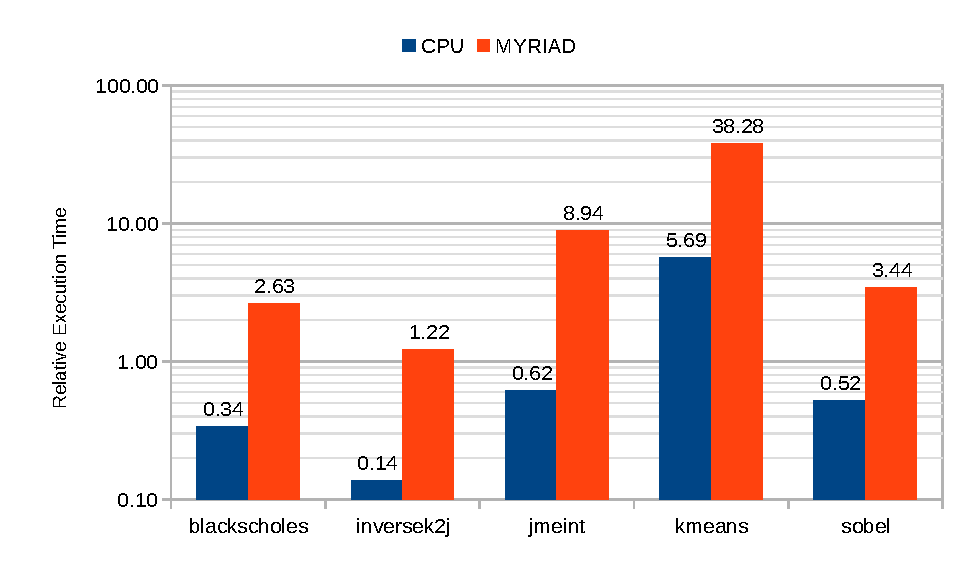
\includegraphics[scale=0.75]{pc_rel_perf}
	\caption{Execution time of the approximate version of the applications relative to the procedural version, tested in a desktop PC.}
	\label{fig:pc_rel_perf}
\end{figure}

Figure \ref{fig:pc_rel_perf_nn_sizes} shows the same results as Figure \ref{fig:pc_rel_perf}, but with three flavors of the same neural network. The first one (NN 1) is the same one as figure \ref{fig:pc_rel_perf}, and constitutes the baseline result. The next two (NN 2 and NN3) are more complex variations with extra layers and extra parameters. Table \ref{tab:nn_topologies} shows the different network sizes. The objective of showing these results is to measure how performance is impacted when using bigger and more complex neural networks. As seen in the graph, blacksholes, inversek2j and sobel were the ones that followed a more lineal trend of complexity vs performance loss, while jmetint and kmeans didn't show much impact in performance relative to the network size. The topologies used for these networks were based on the examples that AxBench includes \cite{Yazdanbakhsh2016}.

\begin{figure}[thbp]
	\centering
	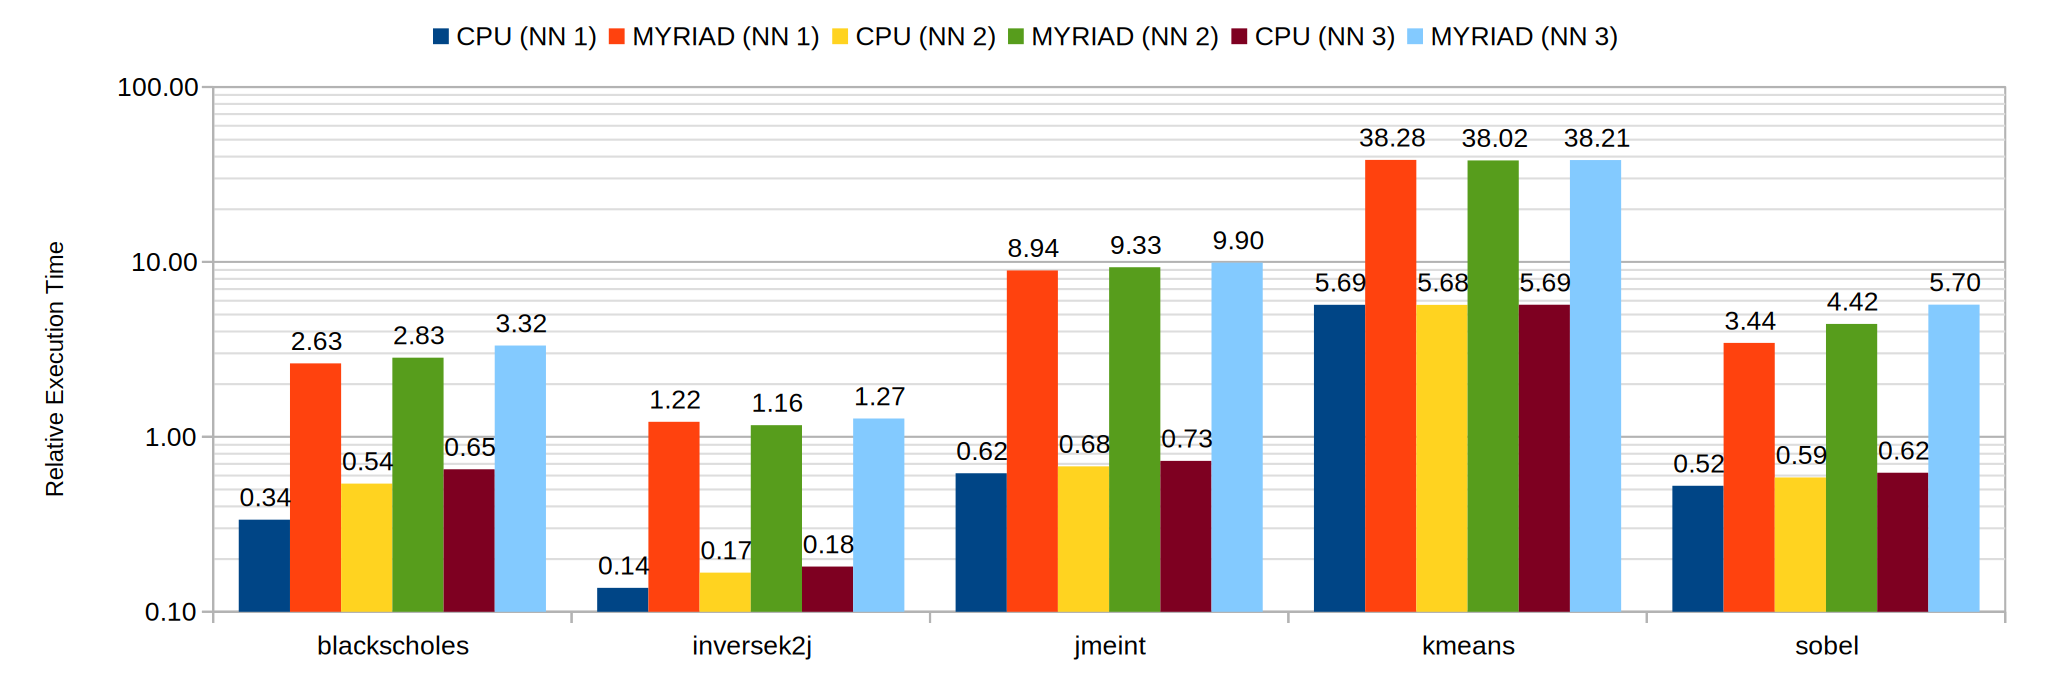
\includegraphics[scale=0.6]{pc_rel_perf_nn_sizes}
	\caption{Comparison of the relative execution time for different neural network sizes.}
	\label{fig:pc_rel_perf_nn_sizes}
\end{figure}

To see how different systems could benefit from utilizing the proposed approximate computing technique, it was tested on three different ones: a PC with an Intel CPU, a Raspberry Pi 3 and a Raspberry Pi 4. One noticeable result was that in the Raspberry Pi 3, the results were lower than expected. One of the reasons is that it only has USB2 ports and it cannot fully utilize the potential of the NCS2. To measure how much the USB2 hurts performance vs utilizing USB3, Figure \ref{fig:usb2} shows the relative slowdown when using USB2 vs USB3 in both the PC and the Raspberry Pi 4. On average, when running in USB3 the performance is 4.6 times better.

\begin{figure}[thbp]
	\centering
	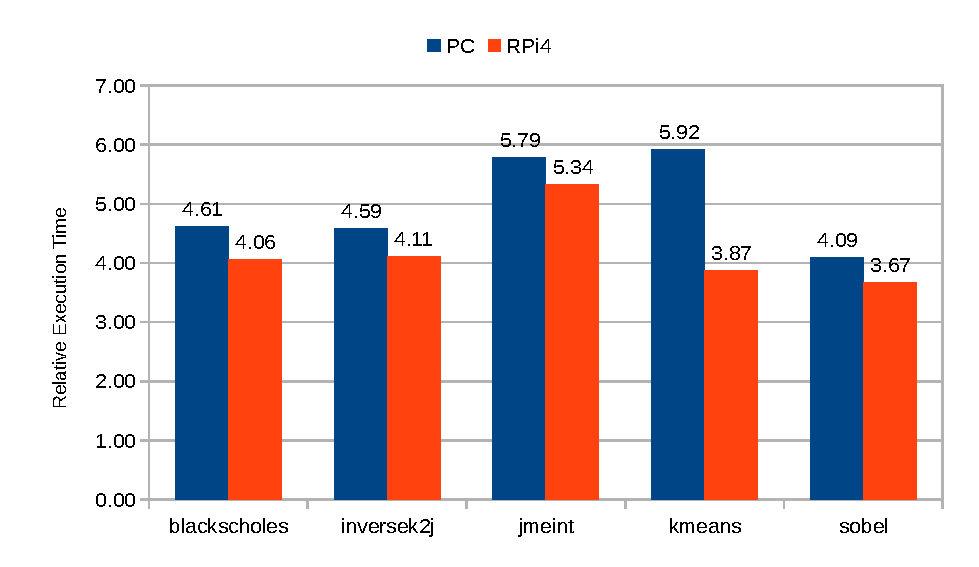
\includegraphics[scale=0.75]{usb2}
	\caption{Slowdown when connecting the NCS2 to a USB2 port.}
	\label{fig:usb2}
\end{figure}

On figure \ref{fig:rpi3_rel_perf} the Raspberry Pi 3 results are shown. Unfortunately, since this system only has a USB2 interface, the system is bottle-necked and most of the applications saw a slowdown compared to the non-approximate version. Only one application, inversek2j, showed an increase in performance using the approximate computing method. Since this system's CPU is slow the relative performance is not as bad as it could be. This shows that any embedded systems that want to benefit from an accelerator like the Myriad need to have a fast interface to reduce bottlenecks.

\begin{figure}[htbp]
	\centering
	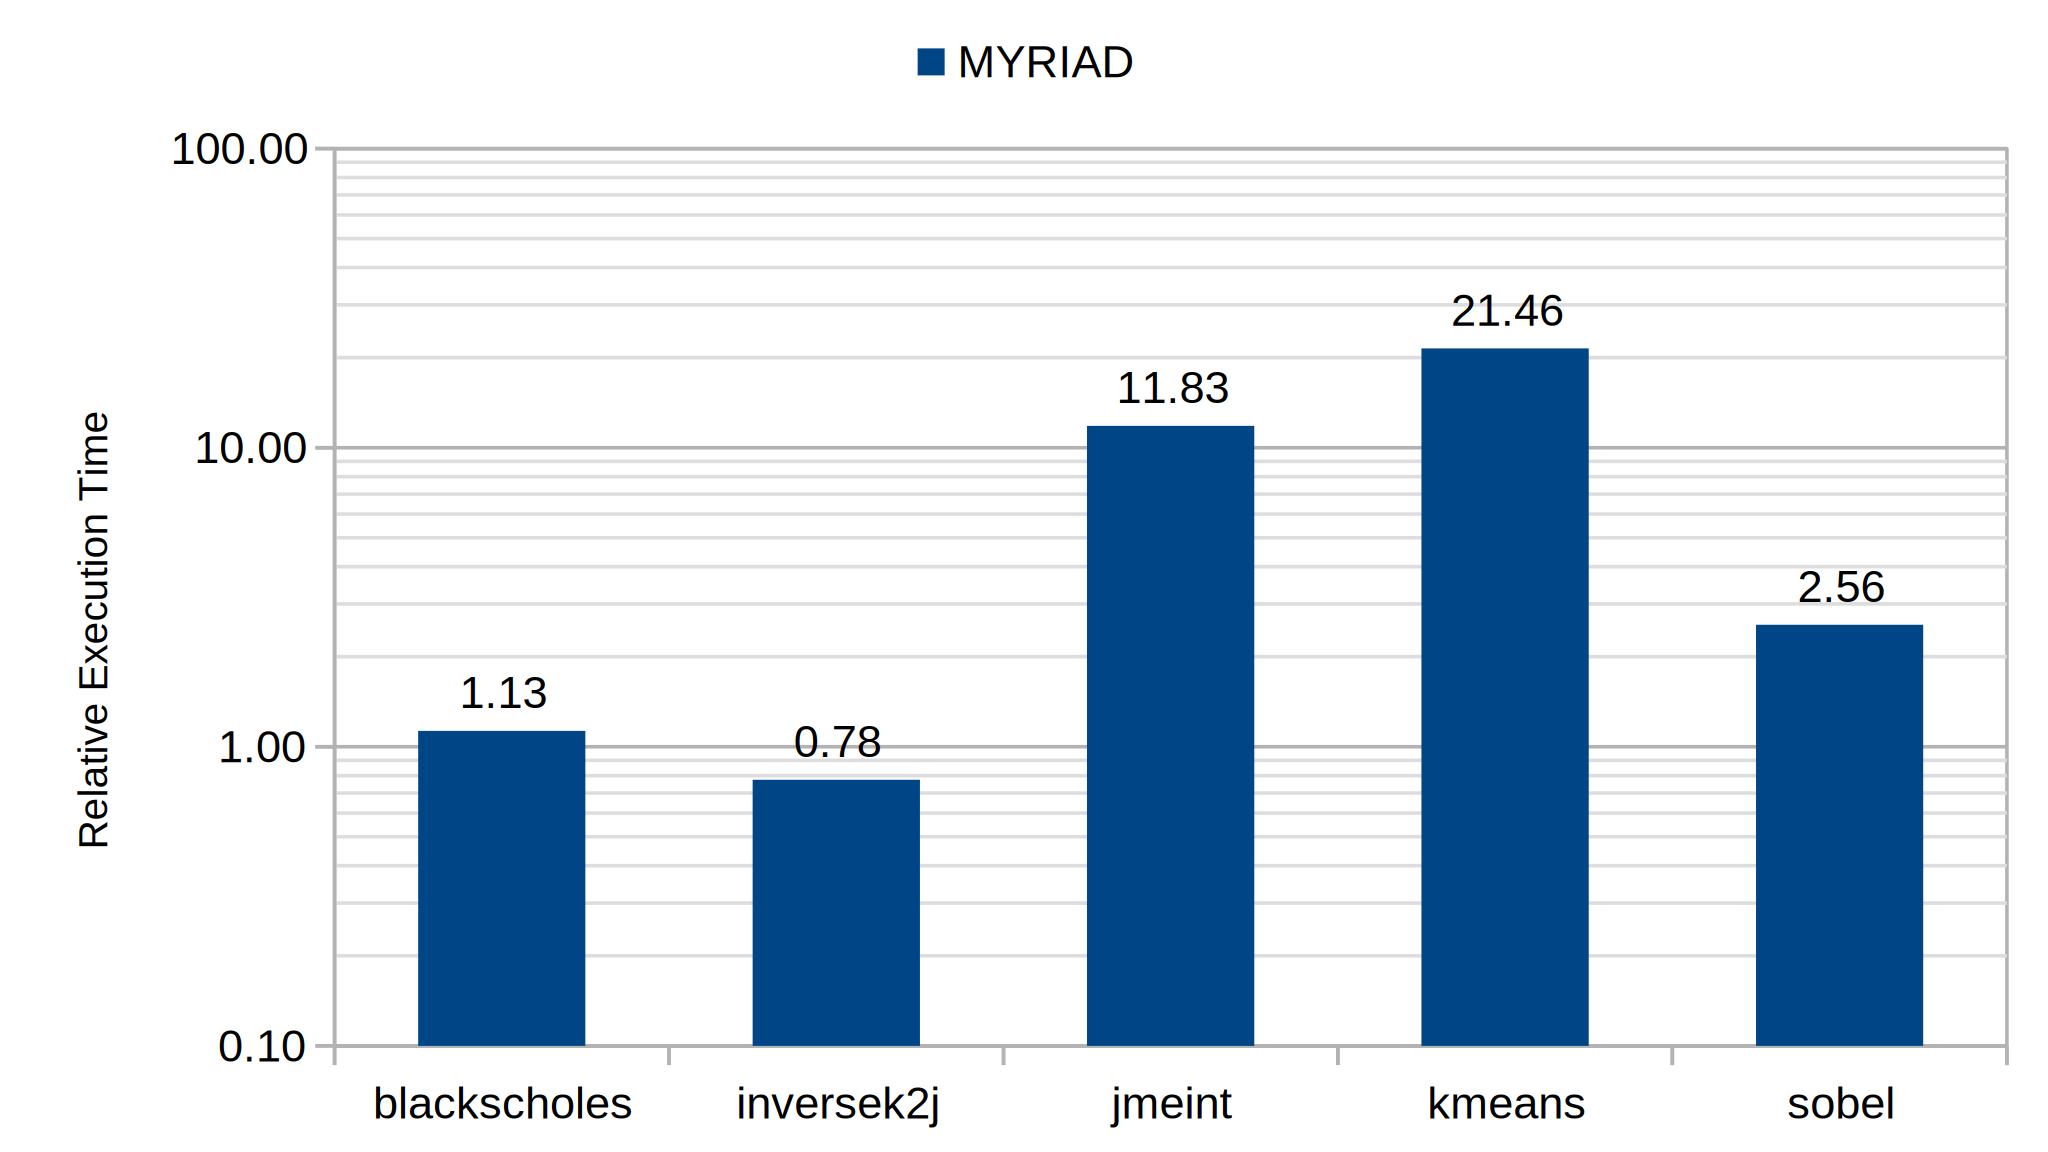
\includegraphics[scale=0.75]{rpi3_rel_perf}
	\caption{Execution time of the approximate version of the applications relative to the procedural version, tested in a Raspberry Pi 3 Model B.}
	\label{fig:rpi3_rel_perf}
\end{figure}

On Figure \ref{fig:rpi4_rel_perf} the results for the Raspberry Pi 4 are shown. Even though this system has a USB3 interface, only two applications showed an improvement in performance. This is because the system contains a CPU that can run the original code much faster. Except for kmeans, all the applications do show a relative improvement in performance compared to the Rapsberry Pi 3.

\begin{figure}[htbp]
	\centering
	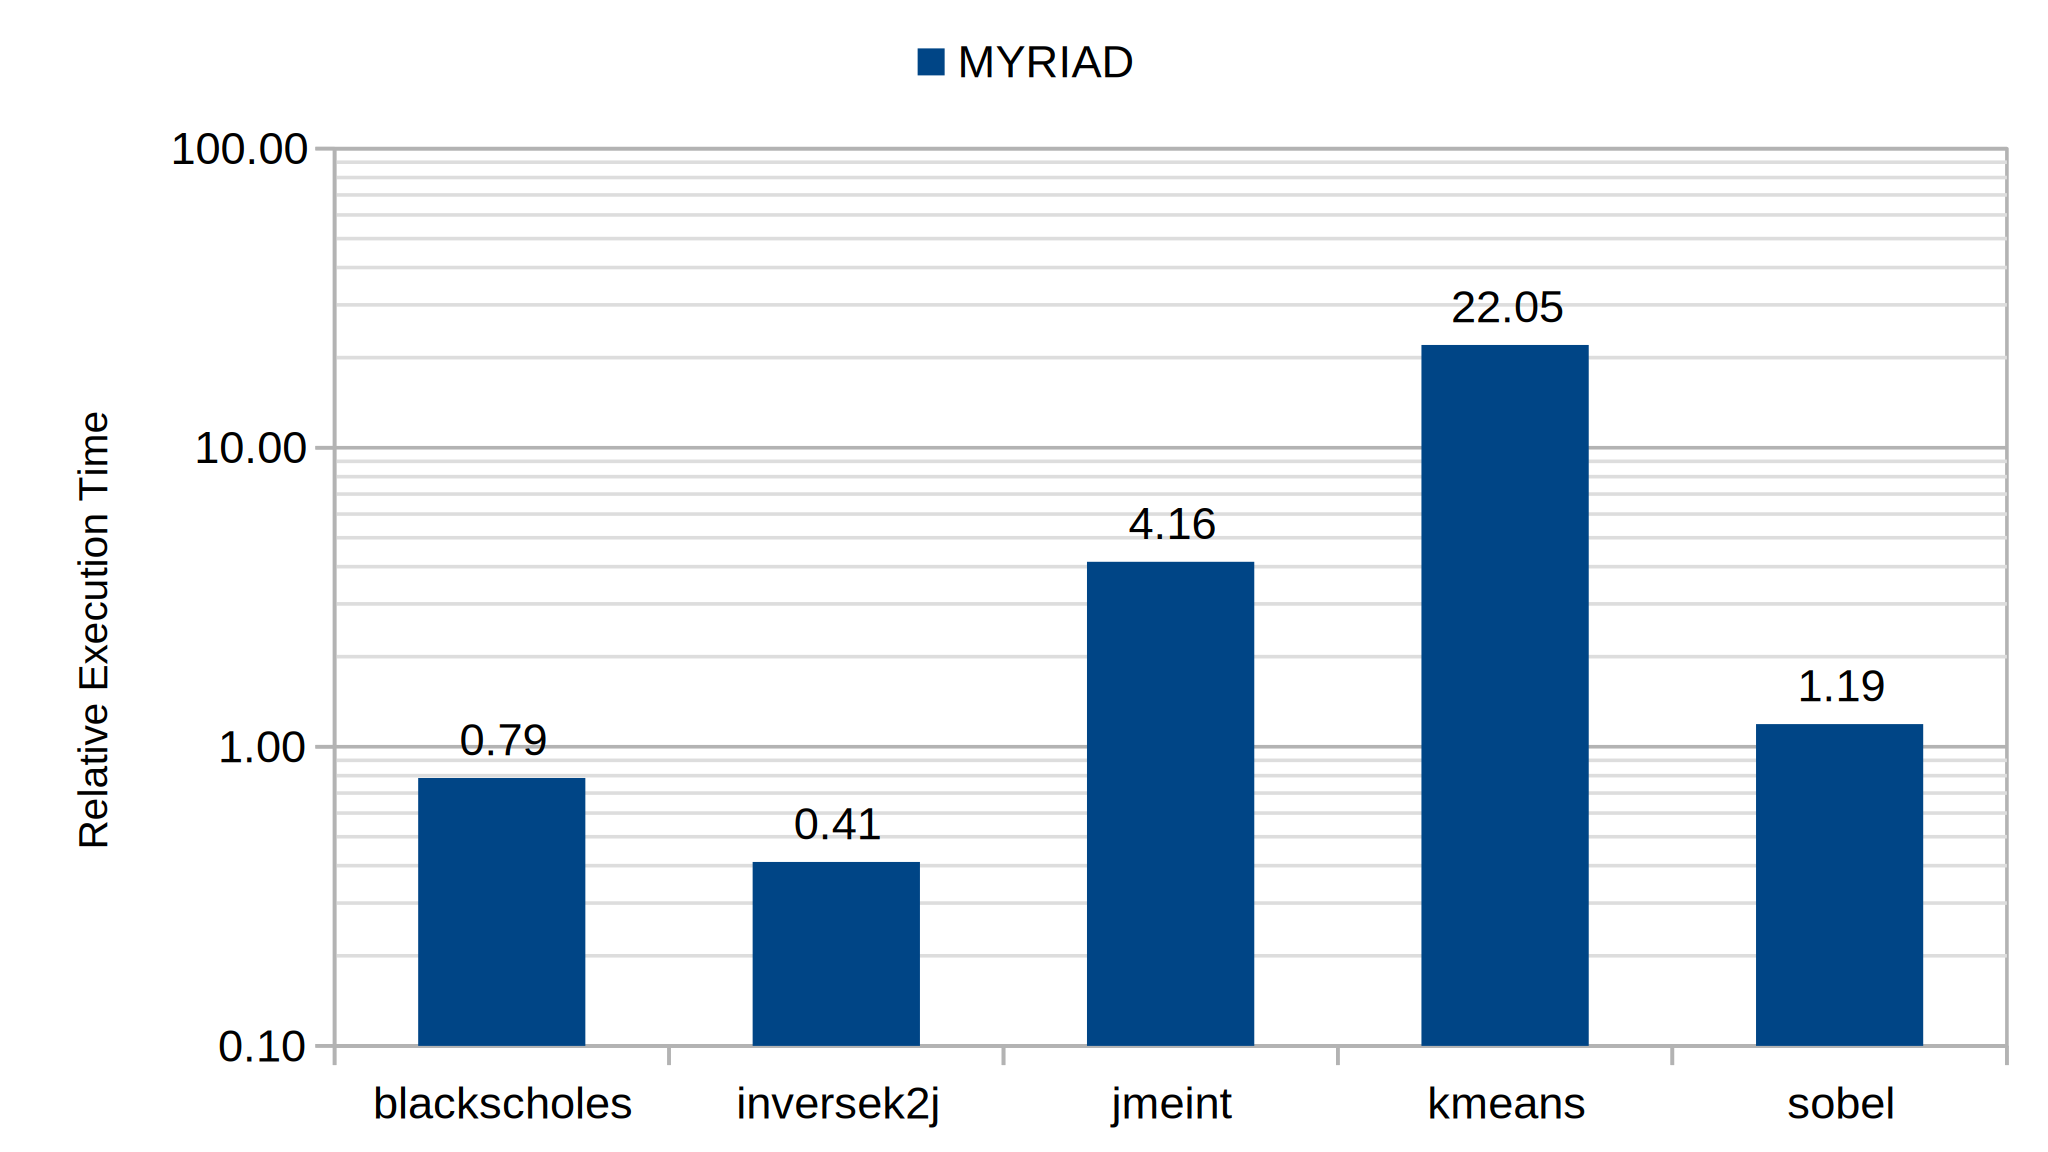
\includegraphics[scale=0.75]{rpi4_rel_perf}
	\caption{Execution time of the approximate version of the applications relative to the procedural version, tested in a Raspberry Pi 4 Model B.}
	\label{fig:rpi4_rel_perf}
\end{figure}

Next the results for the error measurements are shown, starting with the MAPE in Figure \ref{fig:mape}. The graphs for the error measurements all show the three different neural network sizes. Ideally, increasing the size and complexity of the network should reduce the error. The trend mostly follows that assumption, but there are some exceptions. In backscholes, when run in the Myriad VPU, increases in the most complex network. For sobel both the CPU and Myriad results show a degradation in the most complex network. From the graphs it can be concluded that for all the applications except kmeans after the second network there are diminishing returns. This means that there are redundant parameters in the network that are simply not needed or don't contribute significantly to it. The only application that really benefits from a more complex network is kmeans.

\begin{figure}[thbp]
	\centering
	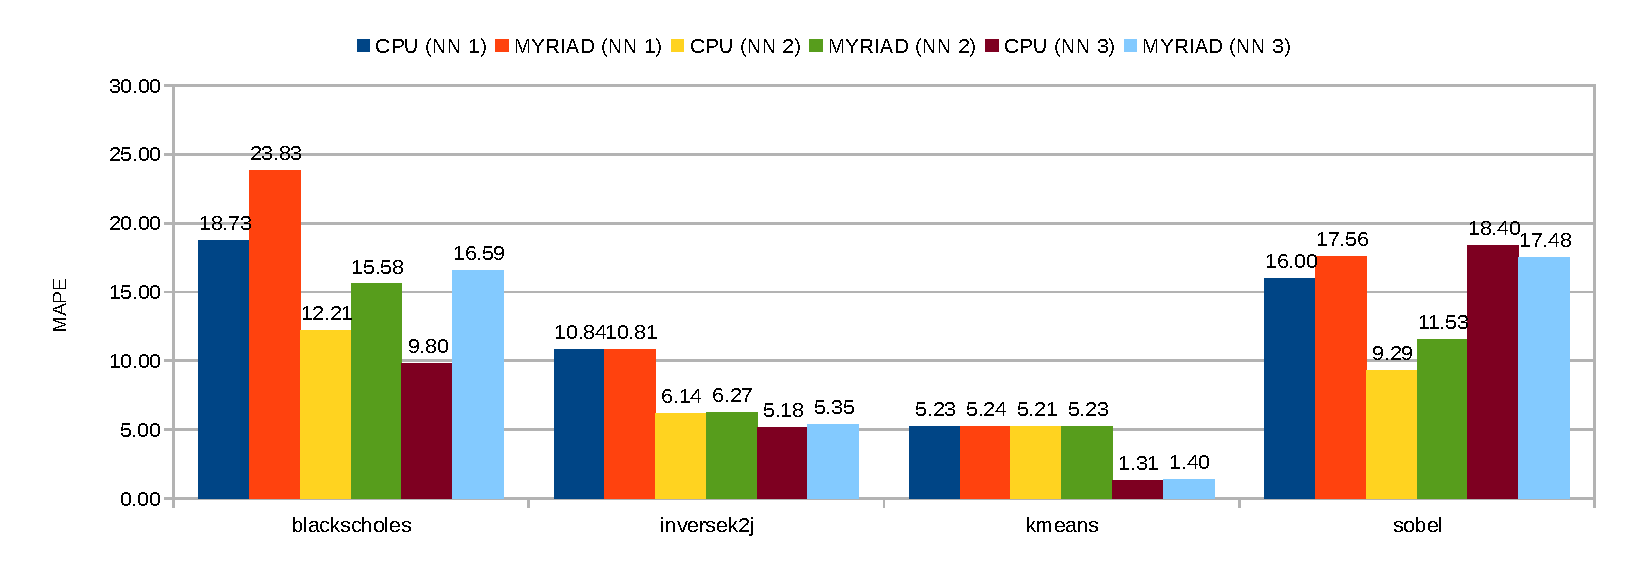
\includegraphics[scale=0.6]{mape}
	\caption{Mean absolute percentage error.}
	\label{fig:mape}
\end{figure}

Figure \ref{fig:wmape} shows the WMAPE and it follows the same trend as the MAPE results. The overall error when measuring the WMAPE is much lower, the reason is that the calculation doesn't punish results that are zero.

\begin{figure}[thbp]
	\centering
	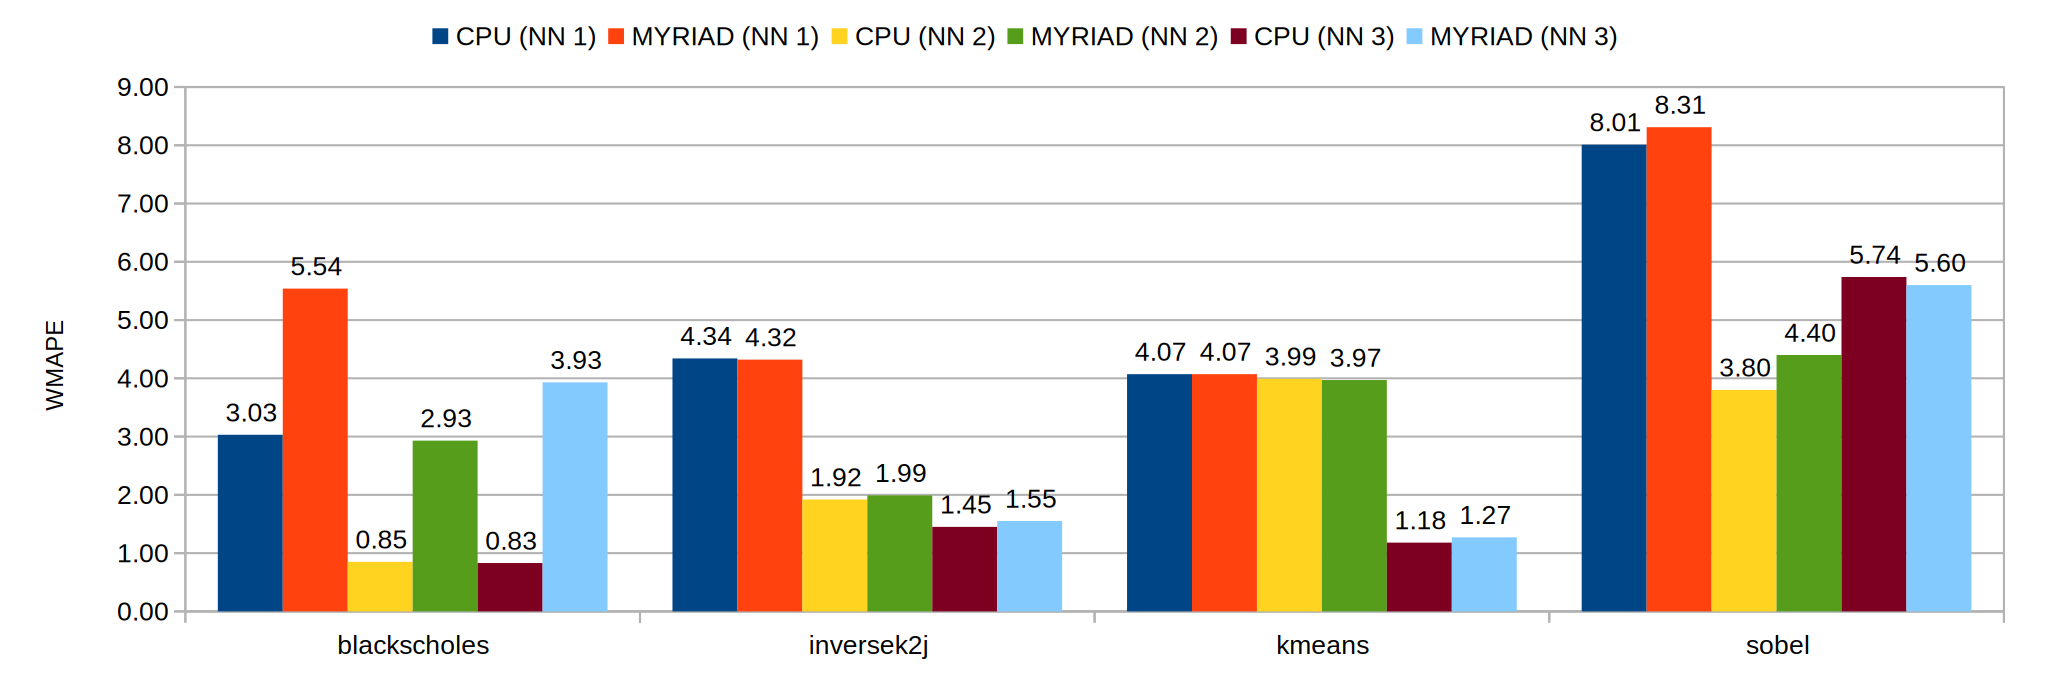
\includegraphics[scale=0.6]{wmape}
	\caption{Weighted mean absolute percentage error.}
	\label{fig:wmape}
\end{figure}

The normalized MSE is shown in figure \ref{fig:mse} and it also follows the same trend as the MAPE and WMAPE results.

\begin{figure}[thbp]
	\centering
	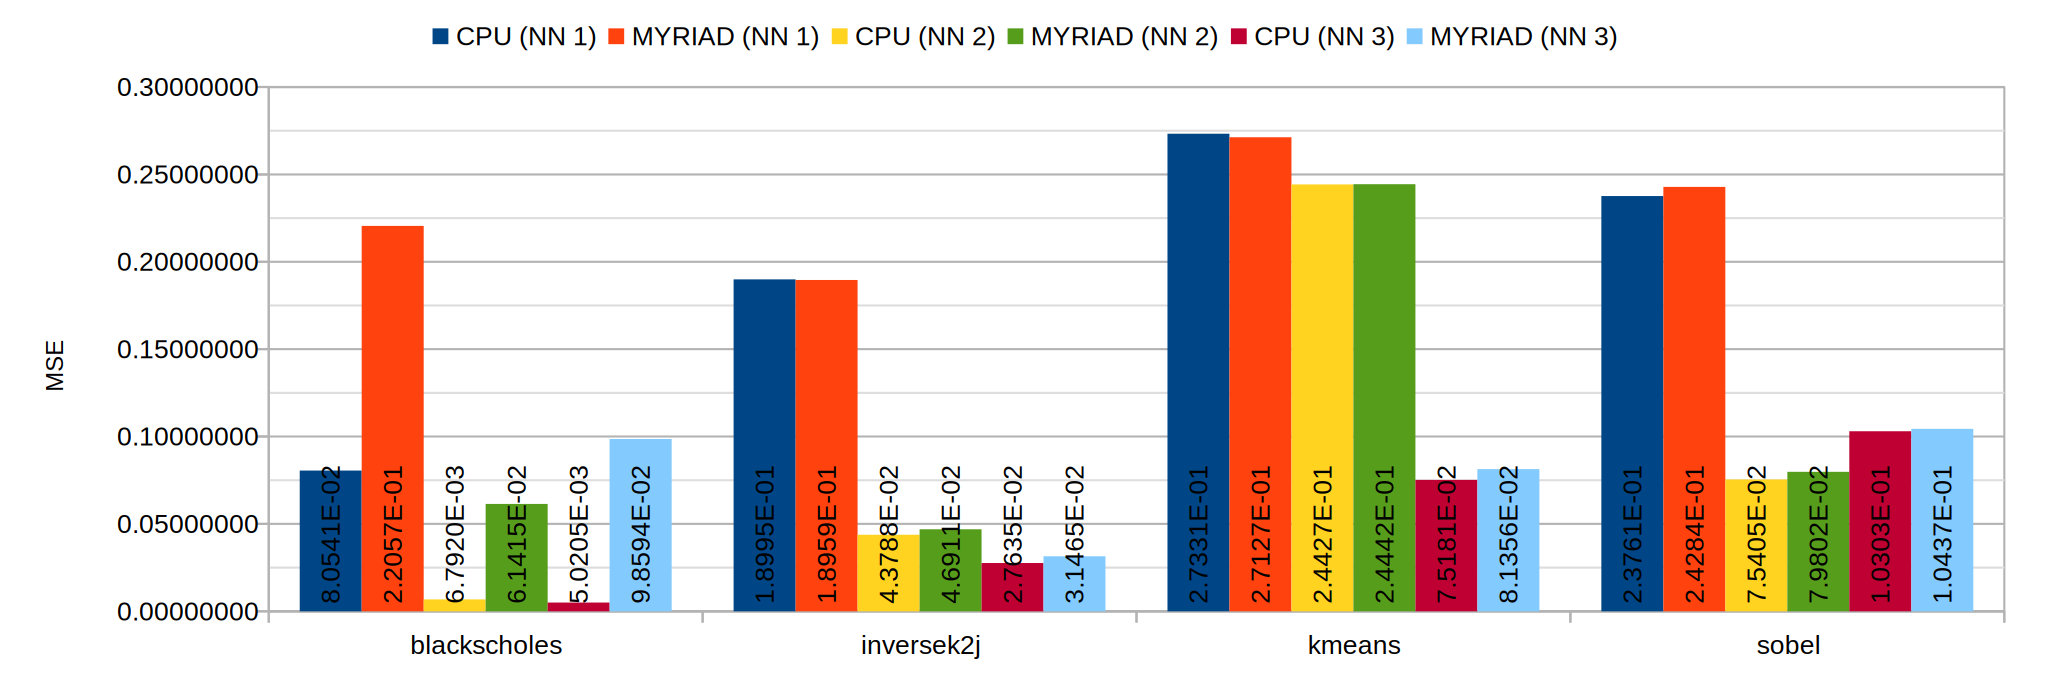
\includegraphics[scale=0.6]{mse}
	\caption{Mean squared error (normalized).}
	\label{fig:mse}
\end{figure}

Figure \ref{fig:perc_err} shows the error for the jmeint application which is measured differently. The results for jmeint are either 0 or 1. The error is the miss rate of the network, the opposite of the accuracy. There is a small benefit of using more complex network, but it shows diminishing returns when the complexity starts to grow.

\begin{figure}[thbp]
	\centering
	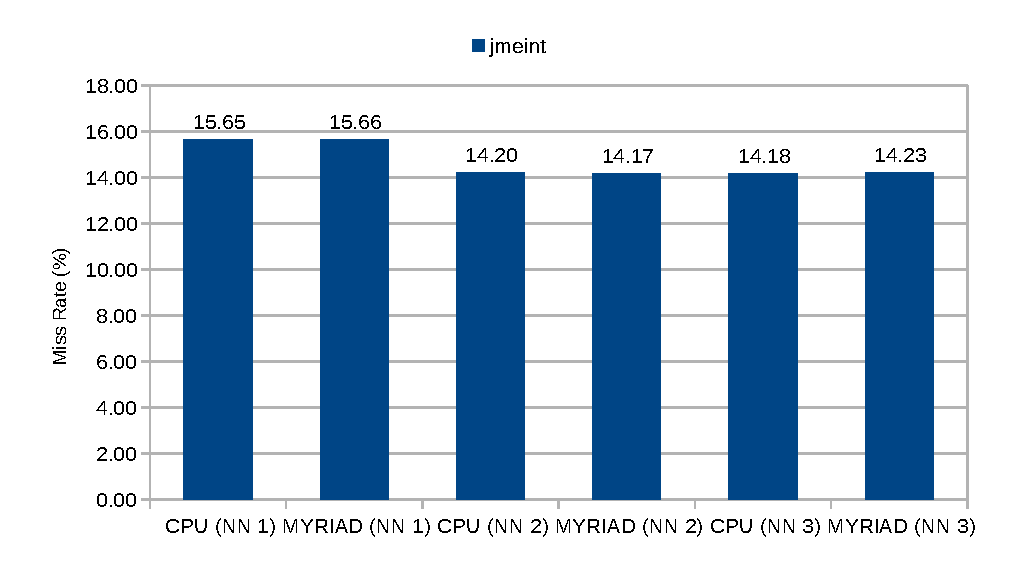
\includegraphics[scale=0.75]{perc_err}
	\caption{Error percentage (miss rate) for jmeint.}
	\label{fig:perc_err}
\end{figure}

In summary, the results were mixed. When using a powerful desktop PC, the results show that using the Myriad accelerator will not improve performance, although its low power could be beneficial in some applications. Using the Intel CPU itself to do the inference can improve the performance since the OpenVINO platform optimizes the model to utilize the CPU efficiently. The most interesting results involve low power platforms like the Raspberry Pi, in which case it is highly recommended that the device supports a high speed interface like USB3, since low speed interfaces significantly reduce the performance by creating a bottleneck when transferring the data. To consider the use of OpenVINO and the Myriad X VPU to accelerate error-tolerant applications thorough benchmarking has to be done to make sure that the specific application can benefit from the capabilities of the toolkit and the accelerator.
%The objective of this chapter was to improve the performance of error-tolerant applications by doing algorithmic transformations that could run in a neural accelerator. This objective was partially achieved since two out of five applications saw an improvement when running in the Raspberry Pi 4.
